\chapter{Data Link Layer - Medium Access Control and Error Control}

\subsection{Coordinated Medium Access}

\noindent
\textbf{Tại sao cần điều phối (coordination)?}
\medskip

\noindent
Khi có nhiều card mạng (network interface card - NIC) cùng kết nối vào một đường truyền chung $\rightarrow$ việc truy cập cần phải được điều phối (need to be coordinated).

$\Rightarrow$ Nếu không có sự điều phối $\rightarrow$ collision sẽ xảy ra khi các thiết bị truyền dữ liệu cùng một lúc.
\medskip

\noindent
$\rightarrow$ Có 2 nhóm phương pháp điều phối.
\medskip

\noindent
\textbf{Contention-based Protocols (giao thức cạnh tranh):}

\begin{itemize}
    \item \textbf{Cơ chế:} các thiết bị tham gia phải cạnh tranh (compete) để truy cập vào đường truyền.
    \item \textbf{Đặc điểm:} \begin{itemize}
        \item Xử lý xung đột (collision handled) $\rightarrow$ do có nhiều thiết bị có thể gửi cùng lúc $\rightarrow$ xung đột là điều chắc chắn xảy ra $\Rightarrow$ protocol phải có cách xử lý chúng.
        \item Non-deterministic (không xác định trước được) $\rightarrow$ không thể biết trước ai sẽ gửi.
    \end{itemize}
    \item \textbf{Hiệu suất:} hoạt động tốt khi lưu lượng mạng thấp đến trung bình, và lưu lượng có tính chất đột biến (bursty).
    \item \textbf{Ví dụ:} ALOHA, CSMA/CA (tránh xung đột bằng cách nghe trước khi gửi - Carrier Sense Multiple Access with Collision Avoidance), MACA.
\end{itemize}
\medskip

\pagebreak

\noindent
\textbf{Contention-free Protocols (giao thức không cạnh tranh):}

\begin{itemize}
    \item \textbf{Cơ chế:} quyền truy cập đường truyền được phân bổ trước (allocated in advance).
    \item \textbf{Đặc điểm:} \begin{itemize}
        \item Tránh xung đột hoàn toàn (collision avoided) $\rightarrow$ collision không bao giờ xảy ra vì đã được plan trước.
        \item Deterministic (xác định trước được) $\rightarrow$ biết rõ ai sẽ gửi và gửi khi nào.
    \end{itemize}
    \item \textbf{Hiệu suất:} hoạt động tốt khi lưu lượng mạng cao (high utilization) $\rightarrow$ đảm bảo tính công bằng (guarantee fair use) về dung lượng mạng cho các thiết bị.
    \item \textbf{Ví dụ:} Token Passing, TDMA (phân chia theo thời gian - Time Division Multiple Access), FDMA (phân chia theo tần số - Frequency Division Multiple Access), CDMA (phân chia theo mã - Code Division Multiple Access).
\end{itemize}
\medskip

\section{Contention-based}

\subsection{ALOHA}

\subsubsection{ALOHA}

\noindent
ALOHA $\rightarrow$ \textbf{A}dditive \textbf{L}inks \textbf{O}n-line \textbf{H}awaii \textbf{A}rea $\rightarrow$ giao thức được phát triển tại Đại học Hawaii vào những năm 1970 để kết nối các trạm từ xa qua sóng vô tuyến.
\medskip

\noindent
\textbf{Pure ALOHA} $\rightarrow$ đây là phiên bản sơ khai và đơn giản nhất.
\medskip

\begin{figure}[h]
    \centering
    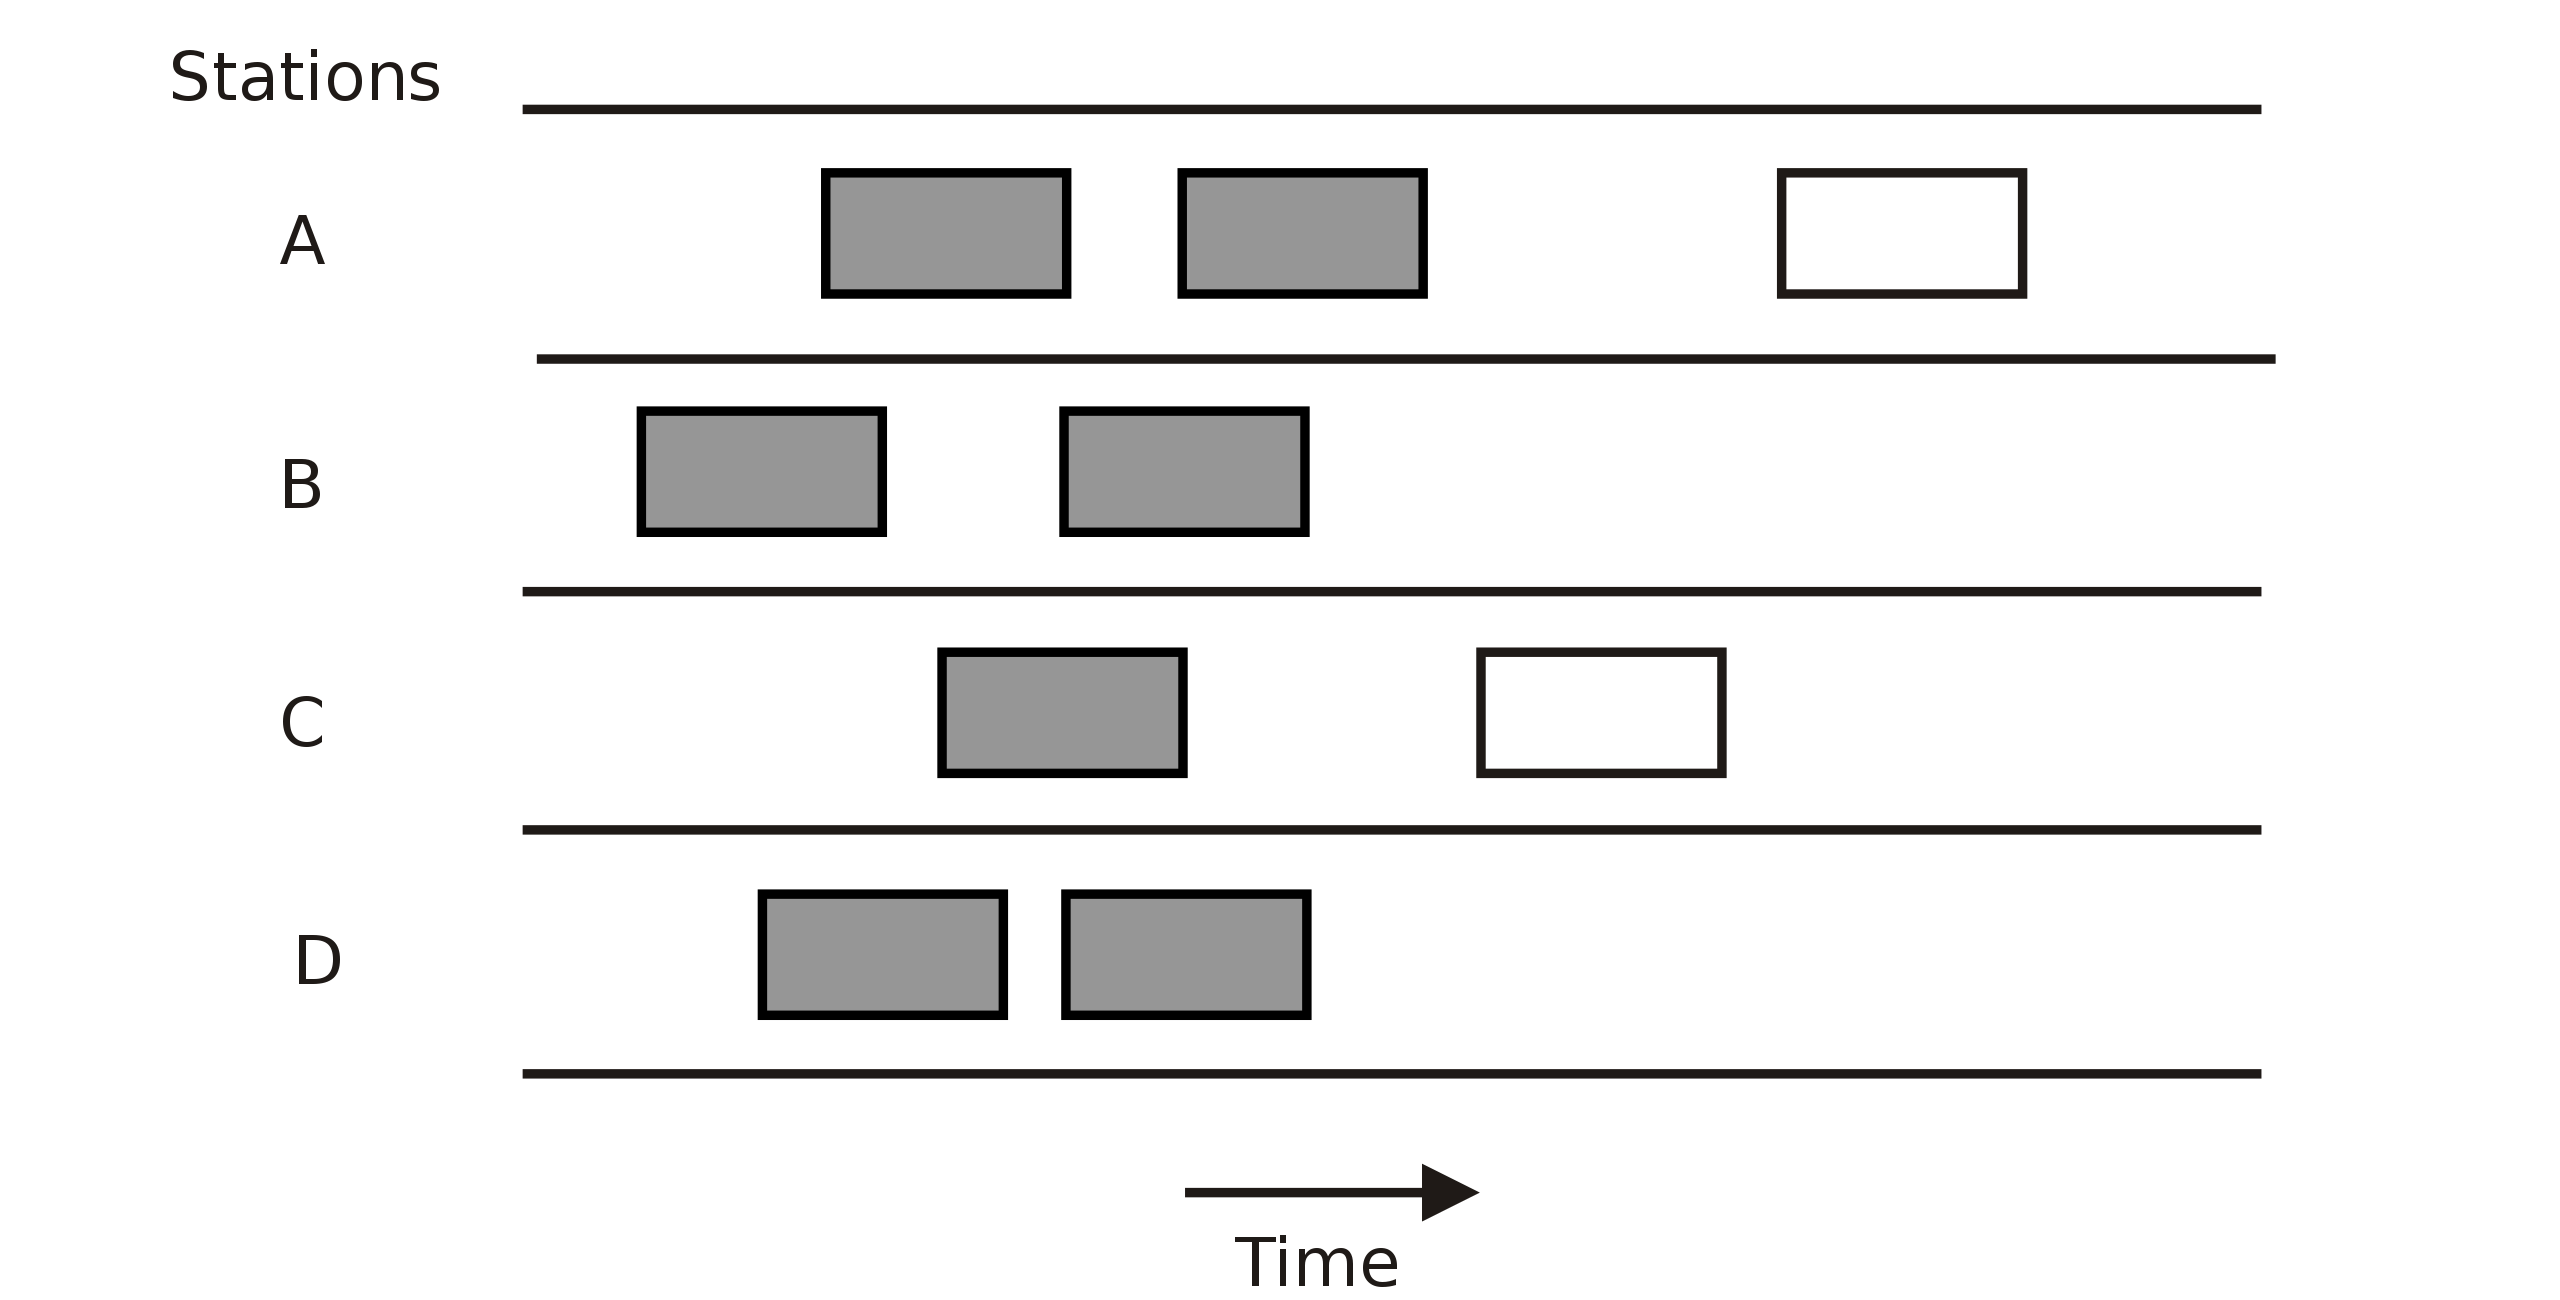
\includegraphics[width=0.6\textwidth]{assets/chap_4/aloha.png}
\end{figure}
\medskip

\begin{itemize}
    \item \textbf{Nguyên lý hoạt động:} không có kiểm soát trung tâm hay sự phối hợp nào giữa các trạm $\rightarrow$ các trạm có thể bắt đầu gửi dữ liệu bất cứ khi nào chúng muốn.
    \item \textbf{Vấn đề:} do ai cũng có thể nói bất cứ lúc nào $\rightarrow$ collision dễ xảy ra $\Rightarrow$ nếu 2 gói tin chồng lên nhau, dù chỉ một chút $\rightarrow$ cả 2 đều bị hỏng.
    \item \textbf{Đặc điểm:} \begin{itemize}
        \item Collision có thể xảy ra \textit{(như nãy nói trên)}.
        \item Không có tính công bằng (no fairness).
    \end{itemize}
\end{itemize}
\medskip

\noindent
$\Rightarrow$ Phương pháp rất đơn giản, không yêu cầu thêm gì.
\medskip
